\documentclass[]{article}
\usepackage[UTF8]{ctex}	% 中文语言包
%\usepackage{multicol}  % 用于实现在同一页中实现不同的分栏
\usepackage{amsmath}	% 公式功能包
\usepackage[shortlabels]{enumitem}	% 编号扩展功能包
\newcommand{\upcite}[1]{\textsuperscript{\textsuperscript{\cite{#1}}}}  % 参考文献设置在右上角


% 伪代码的格式设置
%%***************************************************************************************************
%% 头文件部分
%\makeatletter
%\newif\if@restonecol
%\makeatother
%\let\algorithm\relax
%\let\endalgorithm\relax
%\usepackage[linesnumbered,ruled,vlined]{algorithm2e}%[ruled,vlined]{
%\usepackage{algpseudocode}
%\renewcommand{\algorithmicrequire}{\textbf{Input:}}  % Use Input in the format of Algorithm
%\renewcommand{\algorithmicensure}{\textbf{Output:}} % Use Output in the format of Algorithm 
%%***************************************************************************************************



\usepackage{algorithm}
\usepackage{algorithmicx}
\usepackage{algpseudocode}

\floatname{algorithm}{算法}
\renewcommand{\algorithmicrequire}{\textbf{输入:}}
\renewcommand{\algorithmicensure}{\textbf{输出:}}



\usepackage{titlesec}  % 自定义多级标题格式的宏包

% \titleformat{command}[shape]  % 定义标题类型和标题样式,字体
% {format}  % 定义标题格式:字号(大小),加粗,斜体 例如 \fontsize{20.75pt}\bfseries\centering
% {label}  % 定义标题的标签,即标题的标号等
% {sep}  % 定义标题和标号之间的水平距离
% {before-code}  % 定义标题前的内容

\titleformat{\section}[block]%定义标题类型和标题样式,字体
{\Large\bfseries}  % 定义标题格式:字号(大小),加粗(,斜体),居中
{\bfseries\arabic{section}}  % 定义标题的标签,即标题的标号等
{0.5em}  % 定义标题和标号之间的水平距离
{}  % 定义标题前的内容
[]  % 定义标题后的内容

\titleformat{\subsection}[block]  % 定义标题类型和标题样式,字体
{\large\bfseries}  % 定义标题格式:字号(大小),加粗,斜体
{\bfseries\arabic{section}.\bfseries\arabic{subsection}}  % 定义标题的标签,即标题的标号等
{0.5em}  % 定义标题和标号之间的水平距离
{}  % 定义标题前的内容
[]  % 定义标题后的内容

\titleformat{\subsubsection}[block]  % 定义标题类型和标题样式,字体
{\normalsize\bfseries}  % 定义标题格式:字号(大小),加粗,斜体
{\bfseries\arabic{section}.\bfseries\arabic{subsection}.\bfseries\arabic{subsubsection}}  % 定义标题的标签,即标题的标号等
{0.5em}  % 定义标题和标号之间的水平距离
{}  % 定义标题前的内容
[]  % 定义标题后的内容

\titleformat{\paragraph}[block]
{\small\bfseries}
{[\arabic{paragraph}]}
{1em}
{}
[] 

% \titleformat{\section}[block]{\LARGE\bfseries}{\Roman{section}}{1em}{Hello: }[]
% \titleformat{\subsection}[block]{\Large\itshape\mdseries}{\arabic{section}.\arabic{subsection}}{0.5em}{}[]
% \titleformat{\subsubsection}[block]{\normalsize\bfseries}{\arabic{subsection}-\arabic{subsubsection}}{0em}{}[]
% \titleformat{\paragraph}[block]{\small\bfseries}{[\arabic{paragraph}]}{1em}{}[]



\usepackage{setspace}  % 设置行间距
\usepackage{geometry}  % 设置一些页面格式,还没开发安全
\geometry{a4paper,left=2.0cm,right=2.0cm,top=2.25cm,bottom=2.0cm}

% 正文字体的设置
\PassOptionsToPackage{no-math}{fontspec}
\usepackage{mathspec}
\setmainfont{Times New Roman}  % 正文英文字体的设置
\setCJKmainfont{SimSun}[AutoFakeBold,ItalicFont=KaiTi]  % 正文中文字体的设置
\setCJKsansfont{SimHei}%对应sf无衬线
\setCJKmonofont{FangSong}%对应tt打字机
%\newCJKfontfamily{\kaishu}[AutoFakeBold={2.17}]{STXingkai}


% 摘要格式的设置
\usepackage{tikz}
\usetikzlibrary{shapes,shadows}
\tikzstyle{abstractbox} = [draw=black, fill=white, rectangle, 
inner sep=20pt, style=rounded corners, drop shadow={fill=black,
	opacity=0.5}]
\tikzstyle{abstracttitle} =[fill=white]

\newcommand{\boxabstract}[2][fill=white]{
	\begin{center}
		\begin{tikzpicture}
			\node [abstractbox, #1] (box)
			{\begin{minipage}{0.82\linewidth}
					\setlength{\parindent}{2mm}
					\small #2
			\end{minipage}};
			\node[abstracttitle, right=10pt] at (box.north west) {\textbf{摘要}};
		\end{tikzpicture}
	\end{center}
}
	
	
%\newsavebox{\myabstractbox}
%\providecommand{\abstractnode}[2]{
	%	\begin{tikzpicture}%
		%		\node [abstractbox, fill=#1](box)%
		%		{#2};%
		%		\node[abstracttitle, right=10pt] at (box.north west) {Abstract};
		%	\end{tikzpicture}
	%}
%
%
%\newenvironment{abstractbox][1][white]{
%		\begin{center}%
	%			\def\abs@bgcok{#1}%
	%			\begin{Irbox}{\myabstractbox}
		%				\begin{minipage}{.80\linewidth}%% lparindent2em%
			%					\footnotesize #2
			%				\end{minipage}
		%			\end{Irbox}
	%%			\abstractnode{\abs@bgcol}{\usebox{\myabstractbox}}%
	%		\end{center}%
%	}
		
\makeatletter
\newenvironment{tablehere}
{\def\@captype{table}}
{}

\newenvironment{figurehere}
{\def\@captype{figure}}
{}
\makeatother
		


%opening
\title{一种强大的预训练模型:BERT}
\author{{\small 指导老师:幹泰彬 \quad\quad 周方全 | 202121081229 \quad\quad 研究方向:自然语言处理} }
\date{}



\begin{document}
\maketitle  % 生成标题

%\begin{abstractbox}
%	{\bf 语义切割(Semantic Segmentation)是计算机视觉中十分重要的领域,它是指像素级别的识别图像,即
%		标注出每个像素所属的对象类别。此项技术目前广泛应用于医学图像与无人驾驶等领域。本文主要从语
%		义切割的基本概念介绍在深度学习引入前后此领域的算法发明与改进,侧重点在深度算法,从原始算法
%		全卷积网络(FCN)为切入点,引入一些其改进算法包括:Encoder-Decoder结构的U-net,具有更大感受野
%		的空洞卷积(Dilated Convolution)以及加入条件随机场(CRF)。 \rm} \newline	\newline	
%	{\bf\emph{ Key words-\ 语义切割; 归一化割; 全卷积网络; 空洞卷积; }\rm}	% 文字直接在创建好的环境中输入就可以了。编译后就可以看到效果。
%\end{abstractbox}
\boxabstract{	
%	\kaishu
	{   \textbf{BERT}(Bidrectional Encoder Representation from Transformers)是基于深层Transformer的预训练模型。
		在自然语言呀就领域中,它是一种非常强大的模型,近年来绝大多数自然语言处理的模型都是在其的基础上进行改进优化的。
		BERT不仅充分利用了大规模无标注文本来挖掘其中丰富的语义信息,同时还进一步加深了自然语言处理力模型的深度。
		本文着重介绍在BERT模型中主要成分Transformer模块的数学推导过程以及BERT建模的方法。最后简要介绍使用BERT进行文本分类。 
		\rm} \newline	\newline	
	{   \textbf{关键词-\ BERT; Transformer; 自然语言处理; 文本分类;} \rm}
}
\section{介绍}
在BERT出现之前,无论是基于卷积神经网络还是循环神经网络的语言模型在面对自然语言处理的问题时都是一个浅层的神经网络语言模型。然而,BERT作为一个种非常具有深层思维结构的预测和训练程式语言编程的模型打破了这个壁垒。其“里程碑”的巨大重要性和历史意义就体现在于:不仅证明了针对自然语言处理训练中的分析精度和预测准确率也同样可以通过多次增加数据模型的预测深度而显著地得到提高,模型也同样可以通过对一些无符号标记的海量数据模型进行多次集中预测和训练从而获得,使得模型训练方便。

根据论文\cite{devlin2018bert}的介绍,在相同的任务中BERT模型相比其它模型在准确率上会有明显的提高。BERT的通过巧妙的方式获得文本的上下文信息,从而帮助计算机去理解那些在文章中模棱两可的语言。有时在一段话中我们知道有些词句是这段话的重点,它代表了这段话的主要含义;有时相同的一句话在不同的上下文环境中会有完全不同的意思;有时一句话中代词的理解不过也会是文章的意思发生巧妙的变化。这些在BERT模型中都有了很大程度的解决。下面我们先来介绍一下BERT的整体结构。

\section{整体构架}
BERT的基本模型结构由多层Transformer构成,包含两个与训练任务:掩码语言模型(Masked Language Model, MLM)和下一个句子预测(Next Sentence Prediction, NSP),如图\ref{fig:001}所示。

\begin{figure}[htbp]
	\centering
	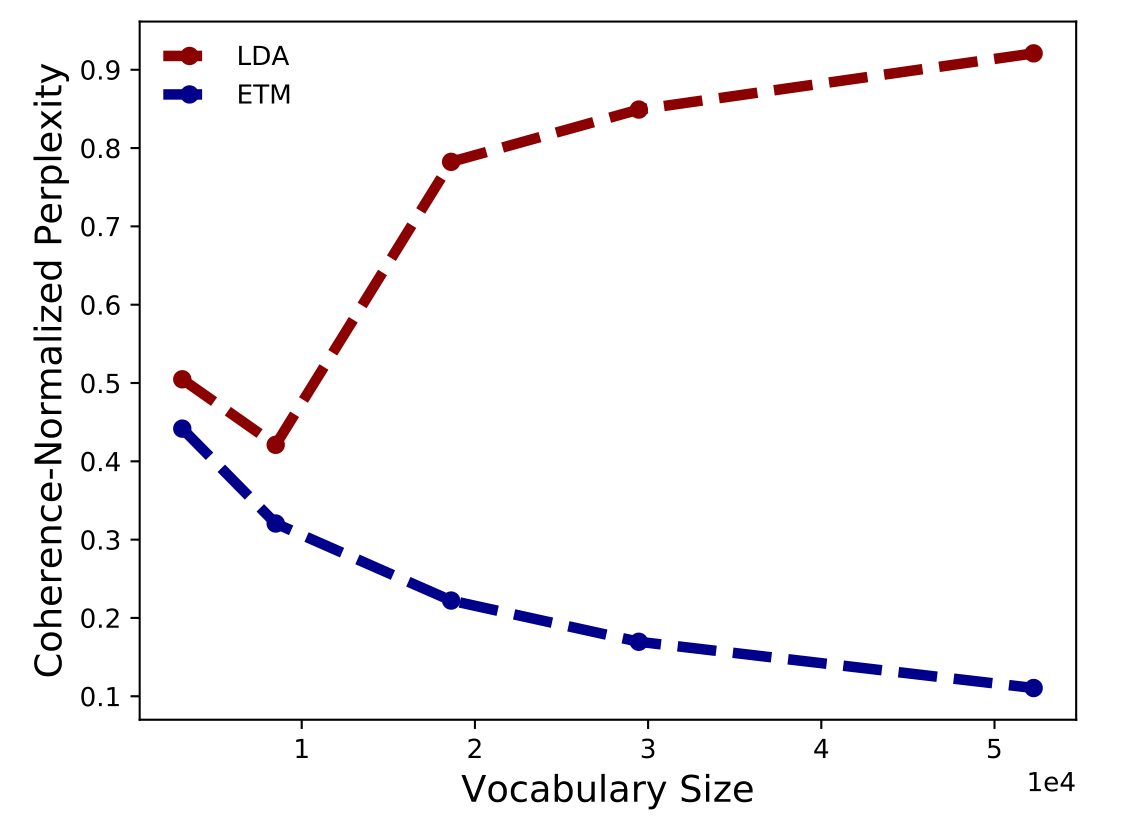
\includegraphics[width=0.6\linewidth]{figures/001}
	\caption{BERT的整体模型结构}
	\label{fig:001}
\end{figure}

可以看到,模型的输入由两段文本 $x^{(1)}$ 和 $x^{(2)}$ 拼接组成,然后通过BERT建模得到上下文语义表示,最终学习掩码语言模型和下一个句子预测。需要注意的是,掩码语言模型对输入形式并没有特别的要求,可以是一段文本也可以是两段文本。而下一步句子预测要求模型的输入是两段文本。因此,BERT在预测训练阶段的输入形式统一为两段文本拼接的形式。接下来我们介绍如何对两段文本建模,得到对应的输入表示。

BERT的 输入表示 由 Token,Segment,和 Position 三部分构成,因为他们要相加,所以单个向量的维度必须是相等的,这样才能相加,如图\ref{fig:002}所示。

\begin{figure}[htbp]
	\centering
	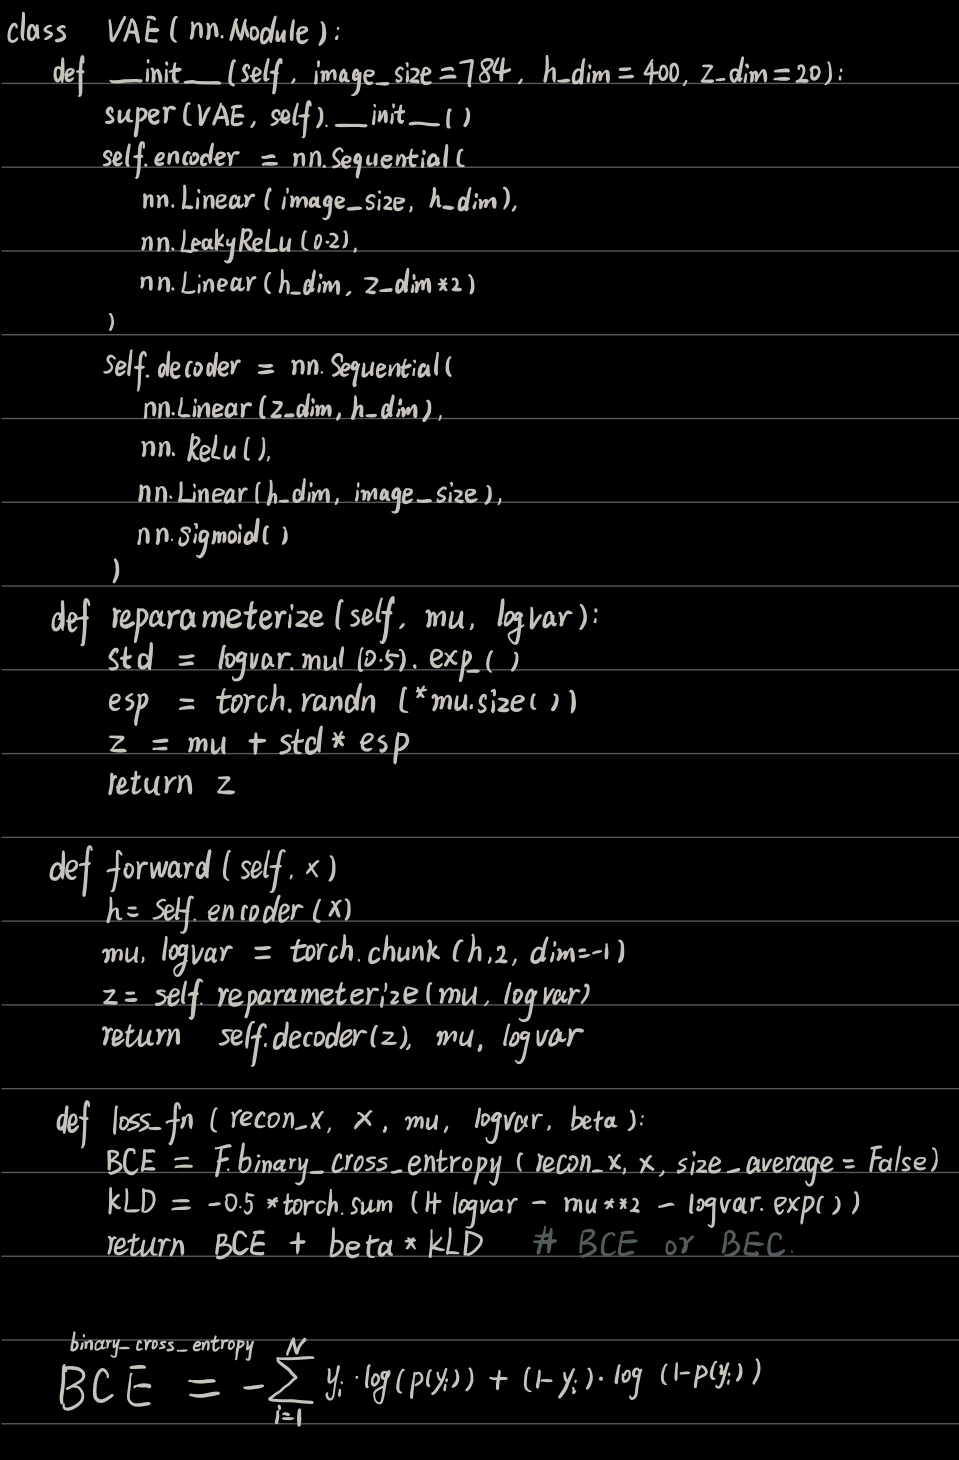
\includegraphics[width=0.6\linewidth]{figures/002}
	\caption{BERT的输入表示}
	\label{fig:002}
\end{figure}

Token 中包括 CLS 和 SEP。CLS 就是 classification,模型最后一层输出的 CLS 提取出来,可以拿他做分类。SEP 就是 separator,用来分隔两段话,放在每段话结尾。因为 NLP 中有的任务是单句输入,有的是多句输入,所以 BERT 为了处理各种任务,设置了 SEP 进行分割,用一套框架就能处理所有任务。

Segment embedding 用来区分每个 token 属于前一段话还是后一段话,是一个可学习的嵌入向量,与 SEP 一起,用来区分不同句子。

BERT 的 Position embedding 与 Transformer 的不同,Transformer 的是由正余弦计算出来的,可以外推,而 BERT 的是个可学习的嵌入向量,学好后维度不能变,没法外推,所以 BERT 会有输入长度限制。

\section{Transformer模块的数学推导}
\subsection{基本模块介绍}
在论文\cite{vaswani2017attention}中提出了Transformer模型,下面我们具体介绍一下Transformer。首先假设Transformer模型就是一个黑箱,我们以机械翻译这个应用为例看看Transformer模型是怎么样工作。如图\ref{fig:003},喂入一个输入,给出一个相应的输出。

\begin{figure}[htbp]
	\centering
	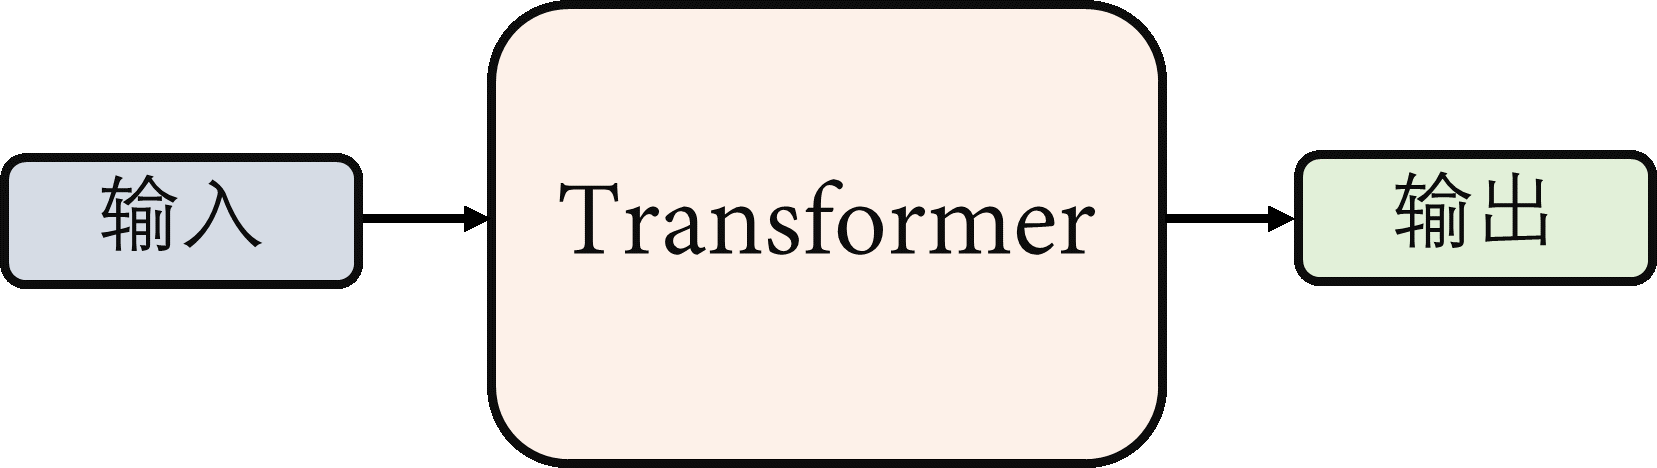
\includegraphics[width=0.6\linewidth]{figures/003}
	\caption{Transformer 模型}
	\label{fig:003}
\end{figure}

我们把这个黑箱展开就会发现里面有两个重要的组件:Encoders和Decoders,以及连接这两个组件的连线。而在Encoders组件中有若干个一样结构的encoder层,同样Decoders组件中也有若干个一样结构的decoder层,如图\ref{fig:004}所示。
\begin{figure}[htbp]
	\centering
	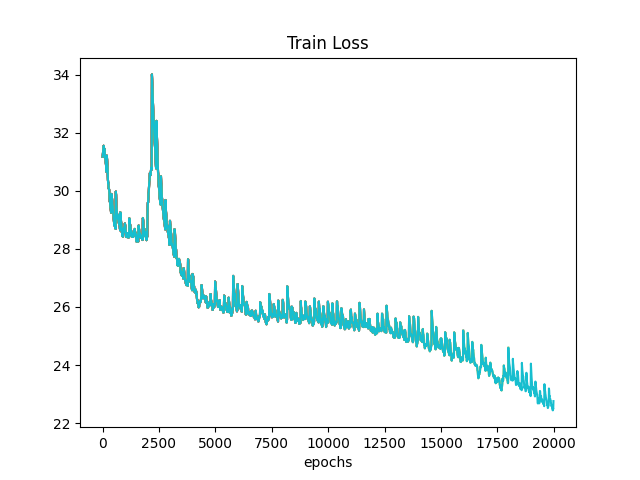
\includegraphics[width=0.6\linewidth]{figures/004}
	\caption{在图中显示的是6个encoder层和decoder层}
	\label{fig:004}
\end{figure}

如图\ref{fig:005},每一个encoder层又可以被细分为两个子层:self-attention层和前馈神经网络层。输入首先经过的是self-attention层,该层帮助编码器在编码特定单词时查看输入句子中的其他单词。该层在后面会进一步讲解。self-attention层输出的数据喂入后面的前馈神经网络层;每个encoder层可以被分成三个子层:self-attention层、attention层和前馈神经网络层。其中第一层和第三层是和encoder层是一样的,中间多加了一个attention层。这个增加的层会使decoder层的注意力分到输入的相关序列上去。
\begin{figure}[htbp]
	\centering
	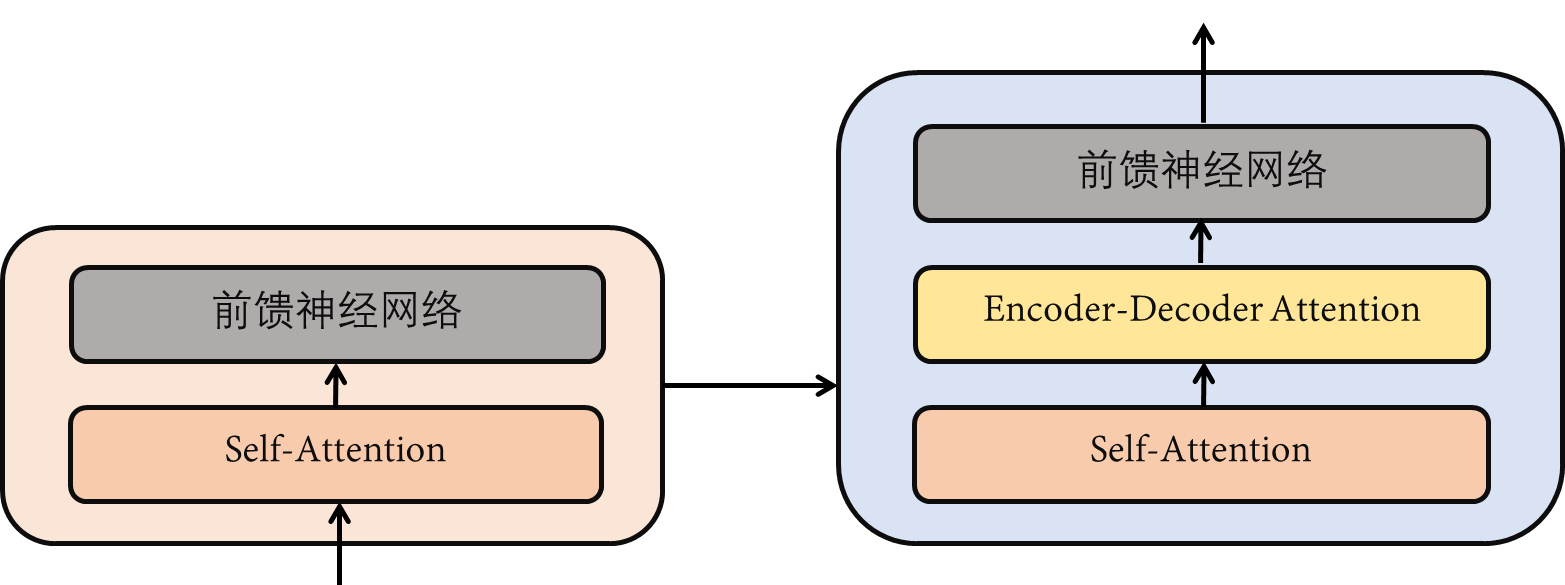
\includegraphics[width=0.6\linewidth]{figures/005}
	\caption{左边是encoder层,右边是decoder层}
	\label{fig:005}
\end{figure}

\subsection{主要模块Self-Attention中的数学推导}

接下来我们来介绍一下在encoder层和decoder层都有的子层Self-Attention层。假设我们对该模型输入一个句子,该句子有$ d $ 个单词,表示为$ S\;{\rm{ = }}\;{\left( {{s_1},...,{s_i},...,{s_d}} \right)^T} $ 。其中$ S $表示一个句子, $ s_i $表示单词。

如图\ref{fig:006}所示。首先,我们使用CWOB将句子$ S $进行编码得到改句子的向量形式X。其中$ {\bf{X}}\; = \;{\left( {{x_1},...,{x_i},...,{x_d}} \right)^T} $,$ x_i $ 表示对每个单词的编码,他们的维度都是一样的。这个维度要看CBOW的设置值,本文设置为常数$ n $ ,故$ {\bf{X}} \in {\Re ^{d \times n}} $ 。而且这个词编码过程只在Encoders组件中第一个encoder层中的Self-Attention层的输入才进行,之后的encoder层的输入不再进行CBOW编码。$ X $经过Self-Attention层后得到输出为$ {\bf{Z}}\; = \;{\left( {{z_1},...,{z_i},...,{z_d}} \right)^T} $ 。之后 $ Z $会进入前馈神经网络层,他的输出会成为写一个encoder层的输入。

\begin{figure}[htbp]
	\centering
	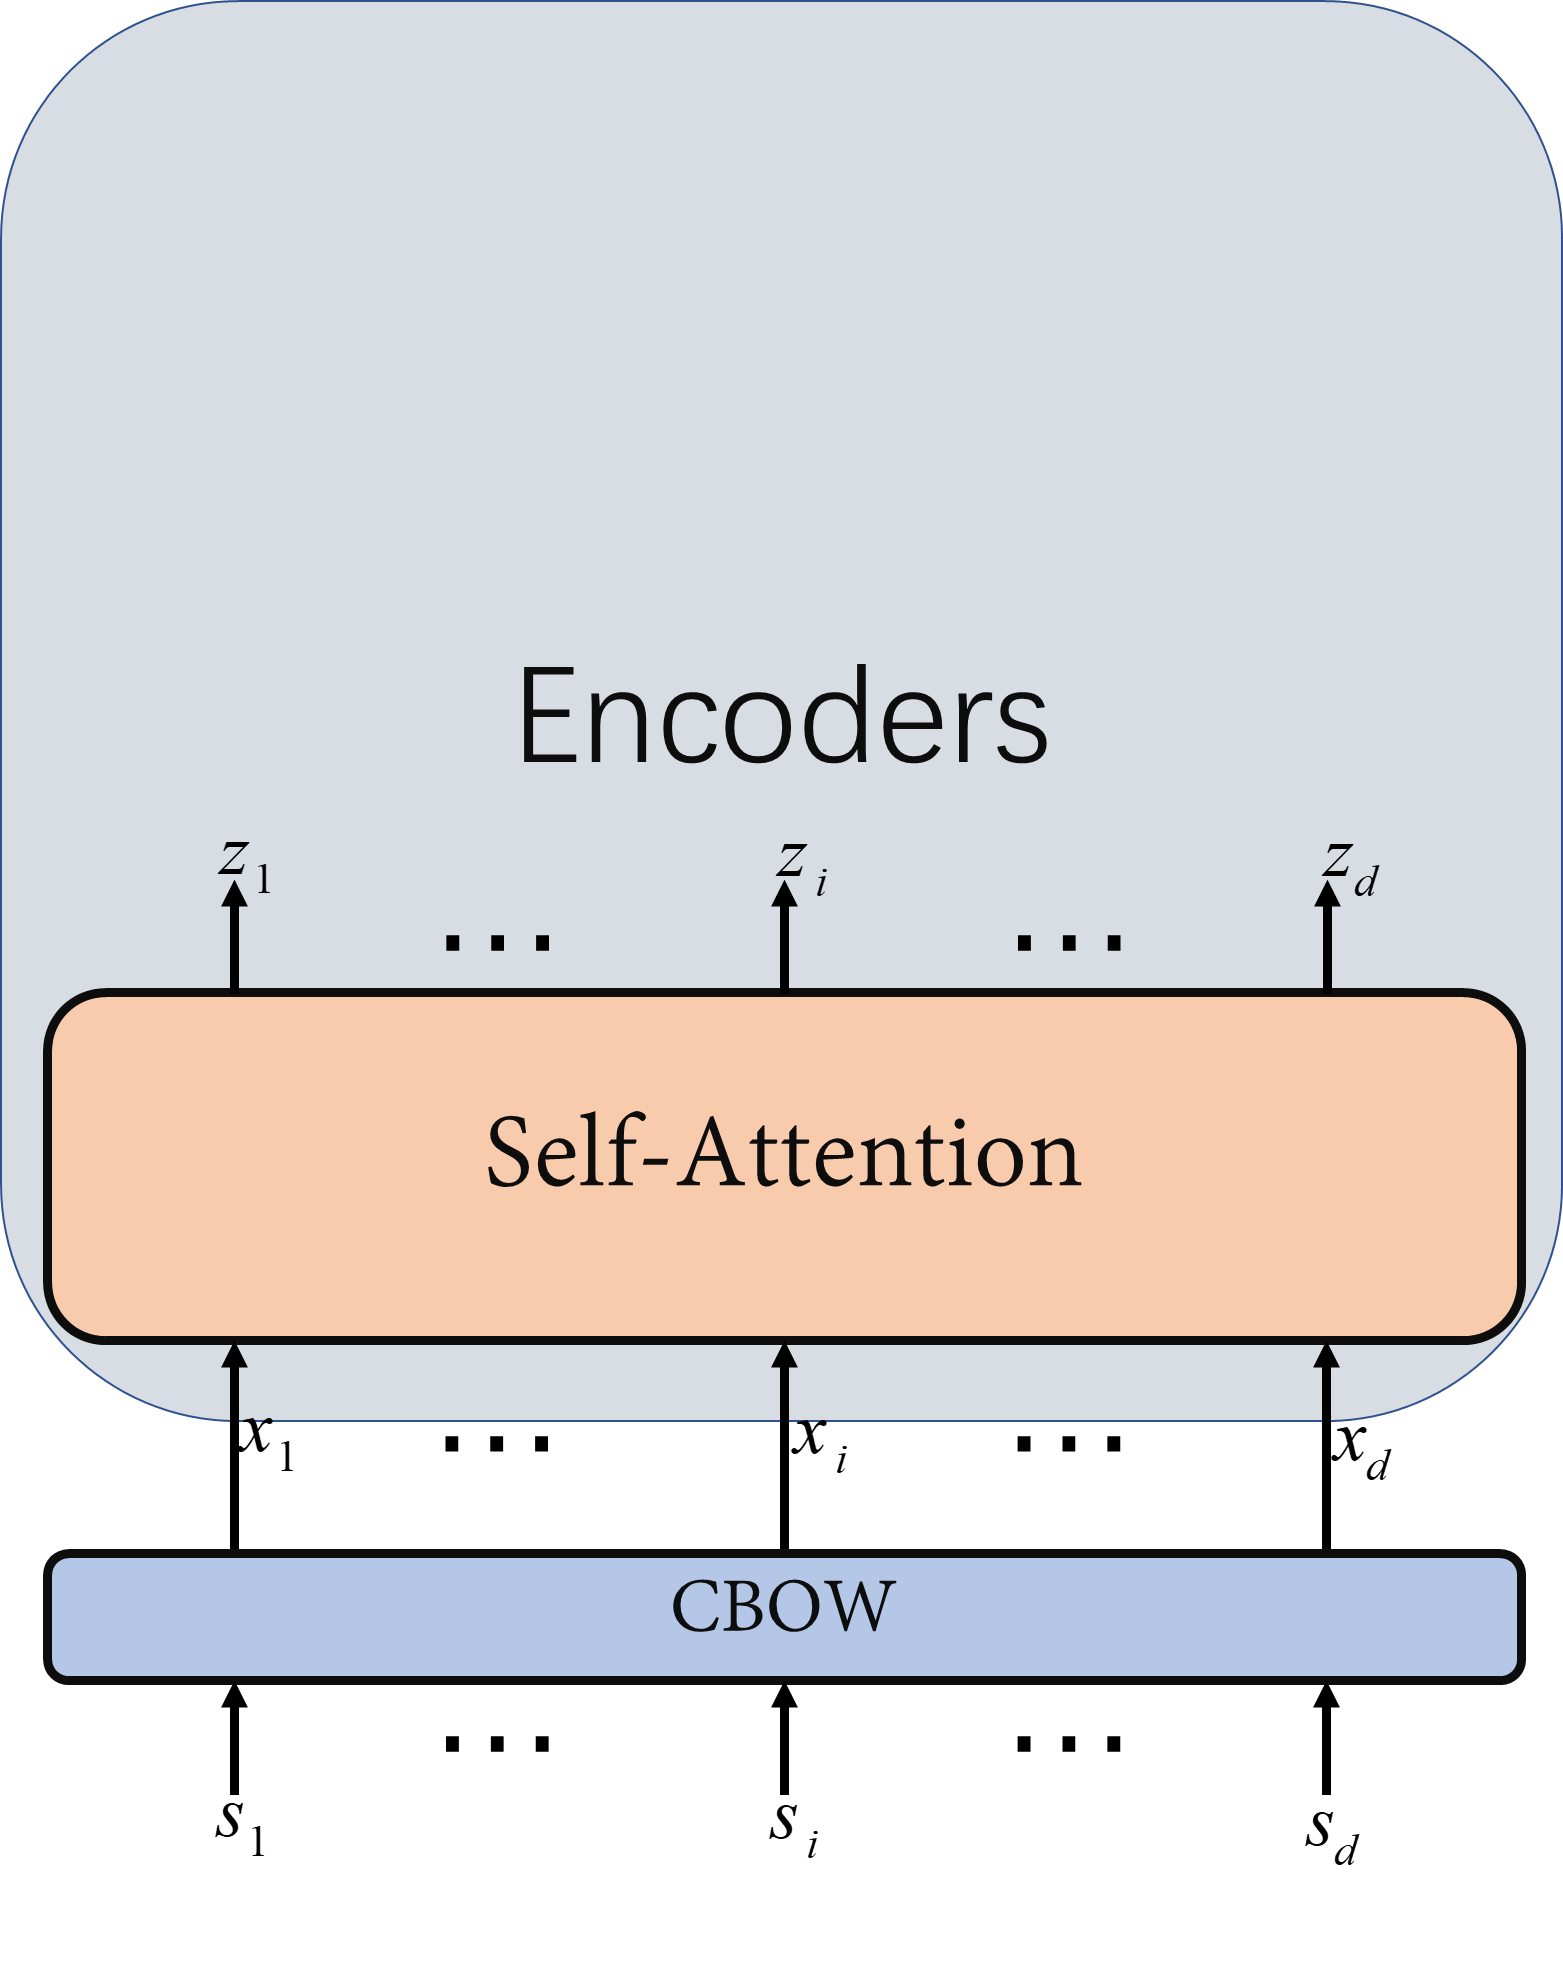
\includegraphics[width=0.6\linewidth]{figures/006}
	\caption{句子$ S $经过CBOW编码得到$ X $,$ X $经过Self-Attention层后得到$ Z $层}
	\label{fig:006}
\end{figure}
由图\ref{fig:006}我们可以直观的看出每一个词在经过Self-Attention层时都有其自己的路径。而且在Self-Attention层中这些路径存在一些依赖关系。而在前馈神经网络层不存在这样的路径依赖关系,因此不同路径在前馈神经网络层的并行计算成为了可能。接下来我们看看在子层Self-Attention中到底是怎么运作的。
由于每个词向量都有自己的路径,所以我们以词向量$ {x_i} \in {\Re ^{1 \times n}} $为例看看在Self-Attention层是如何计算的。如图\ref{fig:007}可以帮助我们接下来四步的计算过程。
\begin{figure}[htbp]
	\centering
	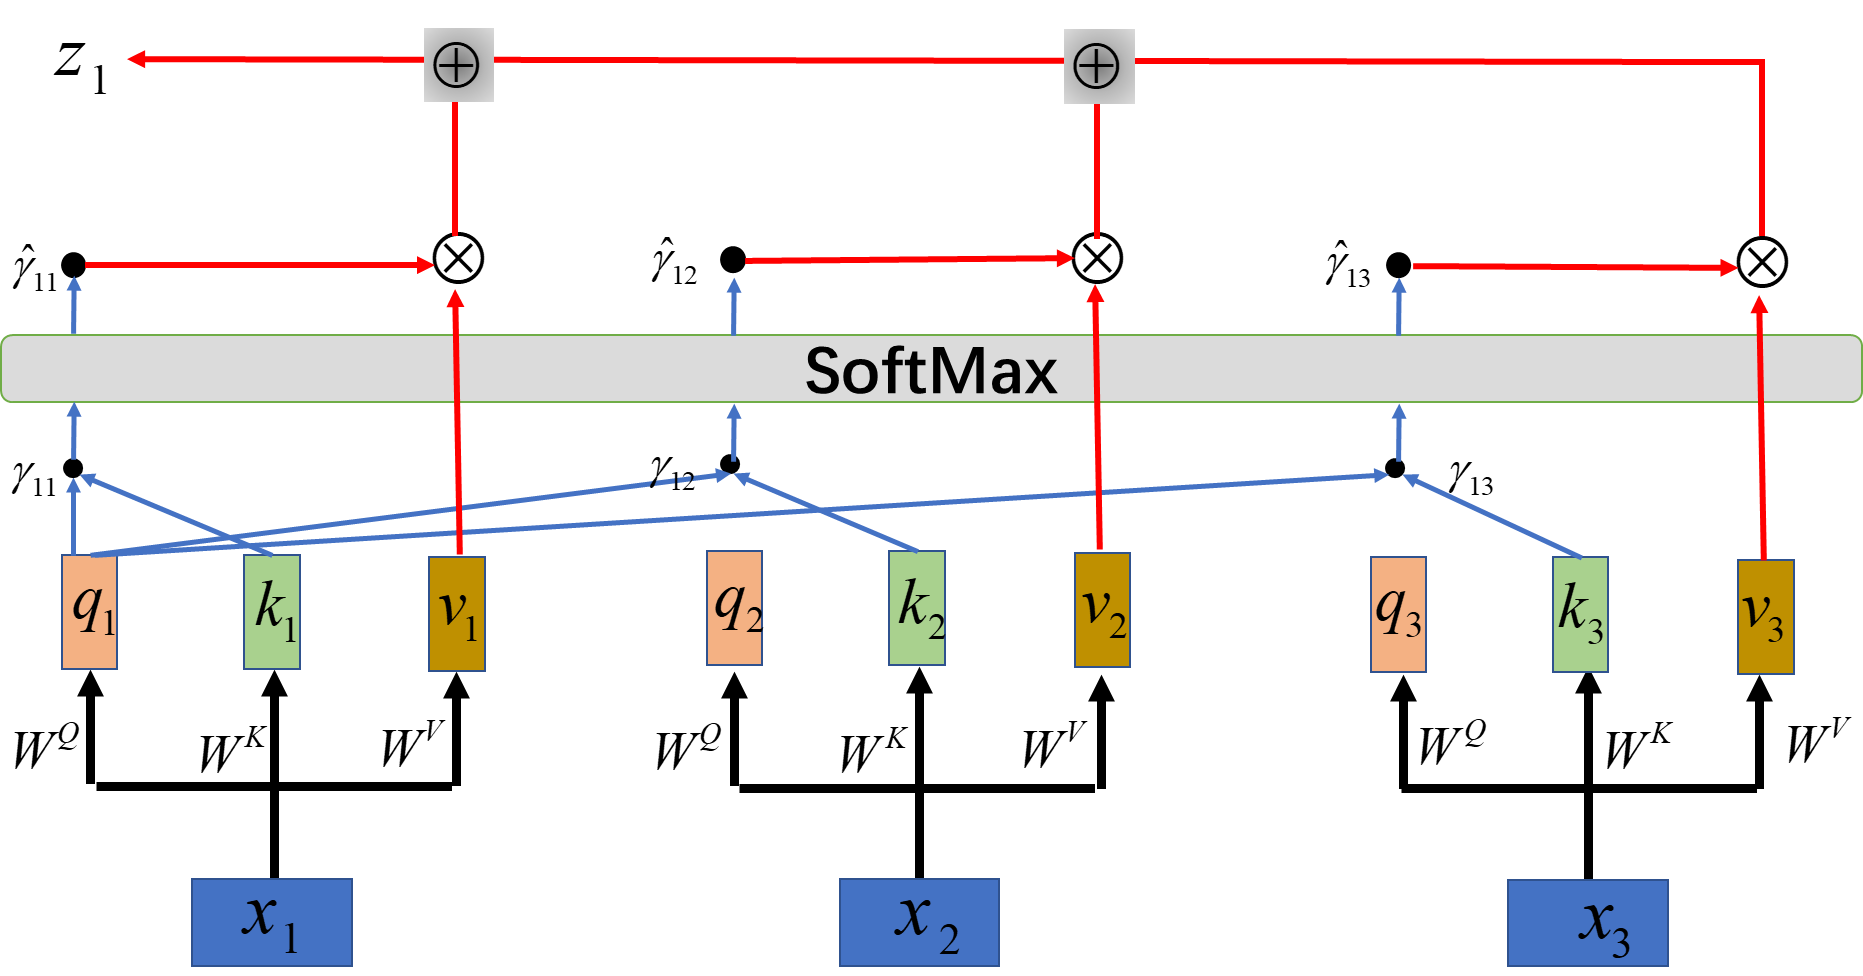
\includegraphics[width=0.6\linewidth]{figures/007}
	\caption{这个句子有3个词,以第一个词向量为例看看其在Self-Attention子层中经过计算得到第一个输出的过程}
	\label{fig:007}
\end{figure}


\begin{enumerate}[i.]
	\item 首先我们设置三个待训练的参数矩阵:Query矩阵${{\bf{W}}^Q}_{n \times m}$ ,Key矩阵${{\bf{W}}^K}_{n \times m}$和Value矩阵${{\bf{W}}^V}_{n \times m}$。他们都是$ m $列的参数矩阵,且所有的词向量公用这三个参数矩阵,一般而言$m \le n$。接着我们用词向量 分别和三个参数矩阵做矩阵相乘得出三个向量:Query向量$ q_i $,Key向量$ k_i $ 和Value向量$ v_i $,其中${q_i}$ 、 ${k_i}$ 、 ${v_i} \in {\Re ^{1 \times m}}$, 。这三个向量是计算和思考注意力的抽象概念。其中 ${q_i}\;{\rm{ = }}\;{x_i} \bullet {{\bf{W}}^Q}$,${k_i}\;{\rm{ = }}\;{x_i} \bullet {{\bf{W}}^K}$ ,${v_i}\;{\rm{ = }}\;{x_i} \bullet {{\bf{W}}^V}$ 。同样,你可以使用相同的方法得到其他词向量的$ q $、$ k $和$ v $。
	\item 我们需要句子中每个单词对该单词进行一个评分,这个评分决定我们在处理这个词向量时,注意力在句子其他部分的关注程度。我们通过公式\eqref{eq:001}计算出我们在处理词向量$ x_i $时,各单词的评分${\alpha _i}\; = \;\left( {{\gamma _{i1}},...,{\gamma _{ij}},...,{\gamma _{id}}} \right)$。其中,$ d_k $是向量$ k_i $的维度。
	\begin{equation}
		{\alpha _i}\;{\rm{ = }}\;{\raise0.6ex\hbox{${{q_i} \bullet \left( {{k_1}^T,...,{k_j}^T,...,{k_d}^T} \right)}$} \!\mathord{\left/
				{\vphantom {{{q_i} \bullet \left( {{k_1}^T,...,{k_j}^T,...,{k_d}^T} \right)} {\sqrt {{d_k}} }}}\right.\kern-\nulldelimiterspace}
			\!\lower0.6ex\hbox{${\sqrt {{d_k}} }$}}
		\label{eq:001}
	\end{equation}
	\item 接着我们将得到的${\alpha _i} \in {\Re ^{1 \times d}}$进行SoftMax处理。即${\hat \alpha _i}\;{\rm{ = }}\;{\rm{SoftMax(}}{\alpha _i}{\rm{)}}$,使得$\sum\nolimits_{j = 1}^d {{{\hat \gamma }_{ij}}} \; = \;1$ 。此时就能很清楚地看出哪个词向量的注意力分配的更多,注意这里的SoftMax是以行为单位进行计算的,这在后面矩阵处理中会用到。
	\item 最后我们将得到的权重${\hat \alpha _i}$分别和${v_i}$进行数乘然后再加得到最后的输出${z_i}$ ,其计算如公式\eqref{eq:002}所示,可知${z_i} \in {\Re ^{1 \times m}}$ ,其中${v_j} \in {\Re ^{1 \times m}}$,${\hat \gamma _{ij}}$ 是一个0~1的常数。这样做会使相关度高的词保留下来,而相关度低的词由于权重太小而被忽略。
	\begin{equation}
		{z_i}\; = \;\sum\nolimits_{j = 1}^d {{v_j} \times {{\hat \gamma }_{ij}}} 
		\label{eq:002}
	\end{equation}
\end{enumerate}

通过上面这四步,我们就得到了词向量$ x_i $经过Self-Attention子层只有得到的输出$ z_i $,继而将得到的结果输入后面的前馈神经网络子层。而在实际的操作中我们并不是一个词向量一个词向量来运算的,而是将一个句子的词向量组成一个矩阵一并送入Self-Attention子层来进行计算。这样就可以实现不同词向量的并行化。针对矩阵的运算我们也有相应的硬件GPU来对矩阵运算进行加速。下面我们看怎么在矩阵层面来进行Self-Attention子层里面的运算。

我们输入一个句子$ {\bf{X}}\; = \;{\left( {{x_1},...,{x_i},...,{x_d}} \right)^T} \in {\Re ^{d \times n}} $矩阵,最后得到$ {\bf{Z}}\; = \;{\left( {{z_1},...,{z_i},...,{z_d}} \right)^T} \in {\Re ^{d \times m}} $。首先我们定义Query向量组$ q_i $,Key向量组$ k_i $和Value向量组$ v_i $组成的矩阵分别是$ {{\bf{Q}}_{d \times m}}{{\bf{K}}_{d \times m}}$和${{\bf{V}}_{d \times m}} $。它们的计算公式如下:

\begin{equation}
	{\bf{Q}}\;{\rm{ = }}\;{\bf{X}} \bullet {{\bf{W}}^Q}
\end{equation}

\begin{equation}
	{\bf{K}}\;{\rm{ = }}\;{\bf{X}} \bullet {{\bf{W}}^K}
\end{equation}

\begin{equation}
	{\bf{V}}\;{\rm{ = }}\;{\bf{X}} \bullet {{\bf{W}}^V}
\end{equation}

然后通过如下公共得出$ {\bf{Z}}\; = \;{\left( {{z_1},...,{z_i},...,{z_d}} \right)^T} \in {\Re ^{d \times m}} $:
\begin{equation}
	{\bf{Z}}\; = \;SoftMax\left( {\frac{{{\bf{Q}} \bullet {{\bf{K}}^T}}}{{\sqrt {{d_k}} }}} \right) \bullet {\bf{V}}
\end{equation}
其中,SoftMax函数对括号里面的矩阵是以行为单位进行计算的。


\section{BERT进行文本分类}
文本分类是多个文本处理应用程序的基础,并被用于许多不同的领域,如市场人力资源、CRM、研究和科学(患者医疗状态分类)、社会网络监控(实时紧急监测、虚假信息发现或任何冒犯性的评论等)。由于深度学习NLP技术的出现,文本分类模型取得了显著的效果,其中BERT模型和其他模型发挥了主导作用。

我们一定想要用BERT开辟的各种可能性。我们有很多方法可以利用BERT的大型知识库来实现我们的NLP应用。
BERT是一个可以微调的模型,我们可以根据自己的任务和特定于任务的数据对模型进行微调,使模型在这样一组特定的参数下能满足我们想要的应用。
那么面对一系列文本我们怎样处理呢?

(1)我们需要把得到的原始文本进行清洗——预处理,将句子中的符号,标点,无实意的词去掉。(2)我们将清洗好的文档结构化。(3)我们将文本输入BERT模型得到相应的词向量编码,由模型得到的高维度的向量表达能力更强,更能显示词与词之间的关系以及次在文本中的关系,所以同样的词但不同的文本环境中得到的词向量编码是不一样的数值。(4)将得到的词向量喂入分类的神经网络,经过训练在得到一个模型参数。这个模型就可以对相应的应用范围批量的对大量文本进行分类。

此外,如果我们的原始数据具有一定的感情色彩标签,那么我们经过训练就可以得到一个可以分析情感倾向的模型。这在餐饮评价,电影评价以及电商的商品评价有很大的应用价值。

\section{展望}
今年来基于词向量语言模型的自然语言处理任务大多离不开BERT,因为它真的很强大。我们对这个模型的依赖在于,它像是一个很好用基础的工具,在此基础上我们可以把原来基于词向量的任务进行优化和提高。再加上近年来深度学习,神经网络风靡一时,以词向量为基础的自然语言任务越来越多,这与能生成高质量的词向量模型BERT相得益彰。除非再出现一个超越BERT的模型,不然它仍会在NLP领域中发挥着无可代替的作用。

\newpage
\bibliographystyle{plain}	% 设置文献样式
\bibliography{sougoul.bib}	% 设置文献的文件路径
\end{document}


